%MIT OpenCourseWare: https://ocw.mit.edu
%RES.18-011 Algebra I Student Notes, Fall 2021
%License: Creative Commons BY-NC-SA 
%For information about citing these materials or our Terms of Use, visit: https://ocw.mit.edu/terms.

\section{Lie Groups}

\subsection{Review}
Last time, we discussed one-parameter groups $G \leq GL_n(\RR).$ We started thinking about tangent vectors to the group, based at some identity.

\begin{definition}
The collection of all tangent vectors at $I \subset G$, called the \textbf{tangent space}, can be characterized in multiple ways. We call this $\lie(G),$ pronounced "lee." 
\end{definition}

\begin{center}
    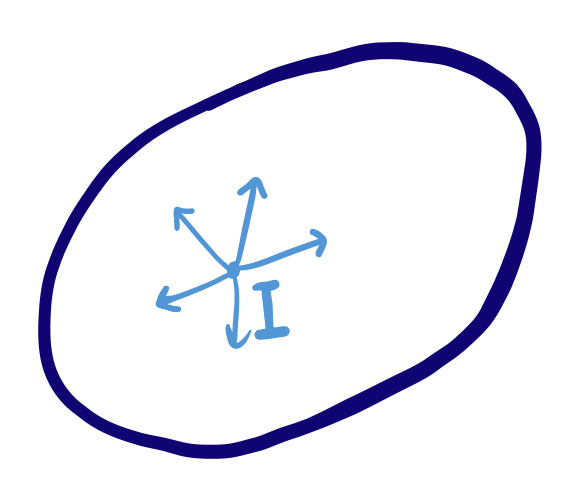
\includegraphics[width=6cm]{Lecture Files and Images/lec33-1.png}
\end{center}

\begin{enumerate}
    \item The first definition is the most familiar one. The tangent vectors are the matrices such that the associated one-parameter subgroup lies in $G$. We found that there is a bijection between matrices and one-parameter groups lying in $G.$ \[\lie(G) = \{A \in \matnn(\RR) : e^{tA} \in G, t \in \RR\}\]
    \item More generally, we consider any path inside the group through the identity, not just a one-parameter group, and take $A$, the velocity at the identity, to be a tangent vector.\footnote{For definition 1, we know all the 1-parameter subgroups, but for definition 2, there are lots of other possible paths. So for definition 1, there is a bijection between the matrices $A$ and the one-parameter groups, while for definition 2, there are lots of different paths with the same tangent vector as the velocity. Definition 2 does not use the fact that $G$ is a group.}
    

    \[\lie(G) = \{A \in \matnn(\RR): \exists f:(-\varepsilon, \varepsilon) \rto G, f(0) = I, f'(0) = A\}\]
    \begin{center}
        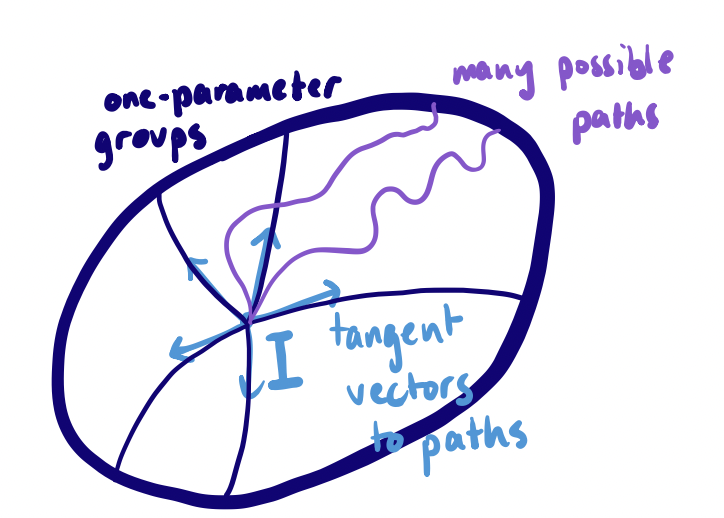
\includegraphics[width=7cm]{Lecture Files and Images/lec33-2.png}
    \end{center}
    \item The third approach is slightly stranger. It is less general, and requires $G$ to be defined by polynomial constraints.\footnote{For example, setting the determinant to be 1 is some complicated polynomial constraint.} In this case, we take this strange construction \[\RR[\varepsilon] = \RR \oplus \RR \varepsilon = \{a + b \varepsilon: a, b \in \RR\},\] where we define the multiplication to be such that \[\varepsilon^2 = 0.\footnote{This is similar to how we could define the complex numbers, where we set $i^2 = -1.$}\] If $f$ is a polynomial, then we can set, formally, the derivative to be \[f'(x) = f(x + \varepsilon) - f(x).\] This is a way of thinking about the derivative without limits, for polnyomials. Then, we take \[\lie(G) = \{A \in \matnn : I + \varepsilon A \text{ satisfies the polynomial constraints defining } G\}.\]
\end{enumerate}

\subsection{Lie Groups}
These definitions are quite abstract, so let's see them in action for $O_n.$ 
\begin{example}
Let $G = O_n,$ the set of matrices such that $A^TA = I.$
\end{example}
\begin{enumerate}
    \item The Lie group, as we have seen in the previous lecture, is \[\lie(O_n) = \{A: A^T = -A\}.\] These are the \textbf{skew-symmetric} matrices.
    \item Consider a path passing through the identity at zero: \[f: (-\varepsilon, \varepsilon) \rto O_n\] such that $f(0) = I.$ By the definition of an orthogonal matrix, \[f(t)^T\cdot f(t) = I.\] Taking the derivative, \[f'(t)^T \cdot f(t) = f(t)^T \cdot f'(t) = 0,\] and taking $t = 0$ gives $A^TI + IA = 0,$ and thus \[A^T = -A.\] So the same condition holds.
    \item The condition that $A^TA = I$ is a set of complicated polynomial conditions. From definition 3), the Lie group consists of matrices $A$ such that \[(I + \varepsilon A)^T(I + \varepsilon A) = I,\] using the rule that $\varepsilon^2 = 0.$ Multiplying this out, \[I + \varepsilon A^T + \varepsilon A + \varepsilon^2 A^TA,\] and taking $\varepsilon^2 = 0,$ \[I + \varepsilon A^T + \varepsilon A = I,\] which implies that \[A^T = -A\] after dividing both sides by $\varepsilon.$
\end{enumerate}

All three definitions lead to the same Lie group, despite being very different. The third definition is useful because it makes sense even without working over the real numbers, and works for any group defined by polynomial constraints!\footnote{The intuition for this third definition is that it is essentially using the Taylor expansion of the path through the identity, and ignoring third order and higher terms.} For example, the Lie group can be defined for orthogonal matrices over finite fields.

Here are some non-obvious facts about these characterizations of the tangent space at the identity. 
\begin{proposition}
For $\lie(G):$
\begin{itemize}
    \item All three definitions are actually equivalent.
    \item For a group $G,$ $\lie(G)$ is actually a vector \emph{subspace} of $\text{Mat}_{n \by n}(\RR).$
\end{itemize}
\end{proposition}

It is surprising that $\lie(G)$ is a vector space, since the matrix exponential does not generally behave well with respect to addition if $A$ and $B$ do not commute.\footnote{Using the first definition, it is not clear that $e^{tA} + e^{tB}$ can be written as $e^{tC}$.}


\subsection{Manifolds}
In order to understand Lie groups, we have to think about the notion of a \emph{manifold.} For this section, the discussion will be less rigorous and precise, and it is okay not to understand all the definitions; we are just providing the flavor of concepts that will show up in later classes.
\begin{definition}
For $M$ a subset of $\RR^n,$ $M$ is a \textbf{(differentiable) manifold of dimension $d$} if for each $x \in M,$ there exists an open set containing $x$ $V \subseteq M$, an open ball $U \subset \RR^d$\footnote{An open ball is a subset of $\RR^d$ of the form $U = \{x : |x| < \delta\}$ for some $\delta.$}, and a continuous (differentiable) bijection $f: U \rto V.$

\begin{center}
    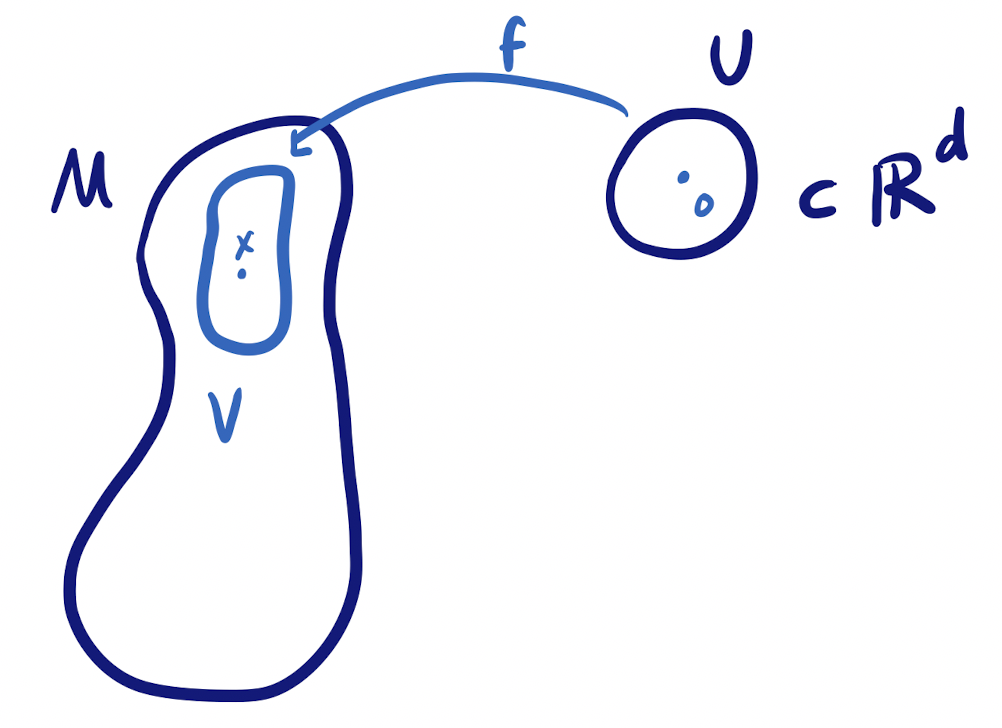
\includegraphics[width=8cm]{Lecture Files and Images/lec33-manifold.png}
\end{center}

\end{definition}



Globally, a $d$-dimensional does not look like $\RR^d,$ but locally, it does. The circle is an example of a 1-dimensional manifold; at each point on the circle, there is really only one direction to move in.


\begin{example}[Circle]

Consider some interval on the real line. Then, it is possible to write down some function bijectively mapping that interval to some other interval on the circle. This can happen around any point on the circle, so it is a manifold.

\begin{center}
    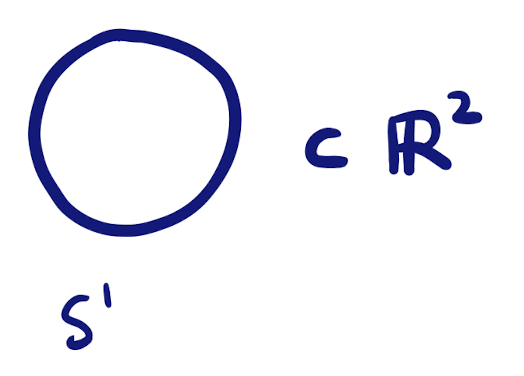
\includegraphics[width=6cm]{Lecture Files and Images/lec33-circol.png}
\end{center}
\end{example}

Loosely, for definition 2, we have tangent vectors at $0$ in $U \subset \RR^d$ corresponding to tangent vectors at $x$ in $M,$ which in a way brings the vector space structure from $\RR^d$ to $M.$ 

A non-example would be the union of the $x$-axis and the $y$-axis, since at the origin, there is an intersection that does not look like an interval. There are two directions to move in, instead of one direction. 

\begin{center}
    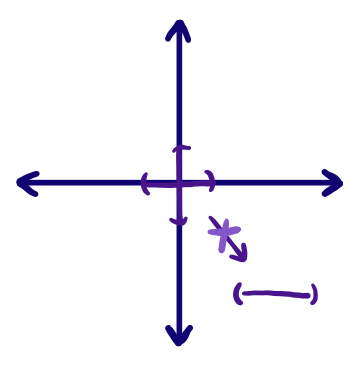
\includegraphics[width=6cm]{Lecture Files and Images/lec33-3.png}
\end{center}


All our examples of $G \leq GL_n(\RR)$ are manifolds, not just groups. This requires some argument, but it is true. 

\subsection{Lie Bracket}

For every group $G,$ there is a corresponding vector space structure $\lie(G) \subset \matnn(\RR) = \lie(GL_n(\RR)).$ In fact, $\lie(G)$ carries some extra structure. The multiplication structure $A, B \rightsquigarrow AB \in \matnn(R)$ does \emph{not} preserve $\lie(G)$; if $A, B \in \lie(G),$ it does \emph{not} mean that $AB \in \lie(G).$ For example, $\lie(O_n) = \{A: A^T = -A\},$ so for $A, B \in \lie(G),$ $(AB)^T = B^TA^T = BA,$ which is not usually equal to $-AB.$ However, a very similar structure \emph{does} preserve the Lie group.

\begin{definition}[Lie Bracket]
Let the Lie bracket of $A, B \in \matnn(R)$ be \[[A, B] \coloneqq AB - BA \in \matnn(R).\]
\end{definition}

% The Lie bracket %idk say something about it

\begin{theorem}
For any $G \leq GL_n,$ the Lie group $G \subseteq \matnn(R)$ is preserved by the Lie bracket:
\[
A, B \in \lie(G) \rightarrow [A, B] \in \lie(G) %probably edit this one lol ?? what does this mean
\]
\end{theorem}

The Lie group is not just a vector space --- it is actually a vector space with some weirdo multiplication on it!

The Lie bracket can be seen in action for some of the Lie groups we have seen already.
\begin{example}
For $G = O_n,$ $\lie(O_n) = \{A: A^T = -A\}.$ Then for $A, B \in \lie(O_n),$ $[A, B] = AB - BA,$ and
\[
[A, B]^T = B^TA^T -A^TB^T = BA -AB = -[A, B].
\]
So $[A, B] \in \lie(O_n).$
\end{example}
\begin{example}
For $SL_n(\RR),$ $\lie(SL_n(\R)) = \{A: \text{trace}(A) = 0\}.$ For matrices $A, B,$ $\text{trace}(AB) = \text{trace}(BA),$ and so $\text{trace}([A, B]) = 0.$ %whats WRONGGGG
\end{example}

The commutator in the group corresponds to the Lie bracket. %what does this mean
\begin{proof}
For $A, B \in \lie(G),$ then consider $e^{tA} \in G$ and $e^{sB} \in G.$ Then we know that 
\[
e^{tA} e^{sB} e^{-tA}e^{-sB} \in G,
\]
and Taylor expanding gives
\[
(I + tA + \cdots)(I + sB + \cdots)(I -tA + \cdots)(I - sB + \cdots) \in G,
\]
which, to the first order, gives 
\[
I + st[A, B] + \cdots \in G.
\]

Then, taking the derivative at $0$ gives 
\[
[A, B] \in \lie(G).
\]%WHO is at 0?? LOL s or t???
\end{proof}

The Lie bracket comes from the fact that the group is closed under multiplication and taking the derivative at 0 for that. As a corollary, if $G$ is abelian\footnote{For example, diagonal matrices}, then the Lie bracket is identically 0 on all of $G.$ In some way, for an arbitrary group $G,$ the Lie bracket "measures" the failure of the group to be abelian. 

We started out with groups that we cared about (matrix groups), looked at the set of tangent vectors, which is the same as the set of one-parameter groups, and looked at the vector space structure which also has a funky Lie bracket, and now we will look at properties of this bracket.

Here are some nice properties of the Lie bracket.
\begin{itemize}
    \item \textbf{Antisymmetry.} $[A, B] = -[B, A]$
    \item \textbf{The Jacobi identity.} We have $[[A, B], C] + [[B, C], A] + [[C, A], B] = 0.$ It is true simply when expanding. This also comes from a property of the group; we won't do it but you can get it by staring at a more complicated version of how we derived the Lie bracket. %explain this better
\end{itemize}

\begin{definition}
A \textbf{Lie algebra} (over $\RR$) is a vector space $V$ with a Lie bracket $[\cdot, \cdot]: V \by V \rto V$ satisfying $[A, B] = -[B, A]$ and the Jacobi identity.
\end{definition}

On the homework, we see that $\RR^2$ with the cross product is a Lie algebra, and it is $\lie(SO_3) = \lie(SU_2).$

If $G$ is a group that is also a manifold, it is called a Lie group, and if $G$ is a Lie group, it can be replaced with $\lie(G)$, a Lie algebra, which is simply a vector space with a weird multiplication on it, which is a lot easier to study. However, the Lie algebra carries a \emph{lot} of information about $G.$ 

\begin{theorem}
Given a Lie algebra (finite dimensional over $\RR$) $V$, there exists a \emph{unique} Lie group $G$ such that $\lie(G) = V.$
\end{theorem}

Lie theory ends up being a very powerful tool in the study of understanding groups.

% Lie groups are symmetries of physical objects no more geometry or group theory. this is step 0 in a whole program of how to ubderstand groups. ok we are done for today.
\newpage